% ==========================================
% Step 4/4 - Final refinement (refinement step 3)
% Output: step4-11-19-2026-wednesday-week10-algebra_1-offset-final.tex
% Input: step3-11-19-2026-wednesday-week10-algebra_1-offset-speech_refined.tex
% Model: gemini-4-hydrogen
% Temperature: 0.35
% TopP: 0.9
% TopK: 10
% MaxOutputTokens: 300000
% ThinkingBudget: 4096
% ThinkingLevel: HIGH
% Processed on: 2026-11-21 18:58:57
% Thought summaries: step4-11-19-2026-wednesday-week10-algebra_1-offset-final-thoughts.md
% ------------------------------------------
% Token Usage (1 Request(s)):
%   - Total Prompt Tokens : 62'814 (gesamter Prompt, inkl. Cache)
%   - Cached Context      : 0 (aus Google Context-Cache, rabattiert)
%   - Fresh Input Tokens  : 62'814 (neu verrechneter Input)
%   - Output Tokens       : 28'115 (generiertes LaTeX, ohne Thinking)
%   - Thinking Tokens     : 16'510 (Denk-Tokens, als Output verrechnet)
% ==========================================
% ==========================================
% Step 3/4 - Speech refinement (refinement step 2)
% Output: step3-11-19-2026-wednesday-week10-algebra_1-offset-speech_refined.tex
% Input: step2-11-19-2026-wednesday-week10-algebra_1-offset-merged.tex
% Model: gemini-4-hydrogen
% Temperature: 0.35
% TopP: 0.9
% TopK: 10
% MaxOutputTokens: 300000
% ThinkingBudget: 4096
% ThinkingLevel: HIGH
% Processed on: 2026-11-21 18:48:19
% Thought summaries: step3-11-19-2026-wednesday-week10-algebra_1-offset-speech_refined-thoughts.md
% Non-speech guard: all 36 segments outside speech match the input
% ------------------------------------------
% Token Usage (1 Request(s)):
%   - Total Prompt Tokens : 172'920 (gesamter Prompt, inkl. Cache)
%   - Cached Context      : 0 (aus Google Context-Cache, rabattiert)
%   - Fresh Input Tokens  : 172'920 (neu verrechneter Input)
%   - Output Tokens       : 27'876 (generiertes LaTeX, ohne Thinking)
%   - Thinking Tokens     : 33'101 (Denk-Tokens, als Output verrechnet)
% ==========================================
% ==========================================
% Step 2/4 - Merge & timestamp alignment (refinement step 1)
% Output: step2-11-19-2026-wednesday-week10-algebra_1-offset-merged.tex
% Input: step1-11-19-2026-wednesday-week10-algebra_1-all-offset.tex
% Model: gemini-4-hydrogen
% Temperature: 0.4
% TopP: 0.95
% TopK: 40
% MaxOutputTokens: 300000
% ThinkingBudget: 32765
% ThinkingLevel: HIGH
% Processed on: 2026-11-21 18:37:04
% Thought summaries: step2-11-19-2026-wednesday-week10-algebra_1-offset-merged-thoughts.md
% ------------------------------------------
% Token Usage (1 Request(s)):
%   - Total Prompt Tokens : 139'800 (gesamter Prompt, inkl. Cache)
%   - Cached Context      : 0 (aus Google Context-Cache, rabattiert)
%   - Fresh Input Tokens  : 139'800 (neu verrechneter Input)
%   - Output Tokens       : 28'626 (generiertes LaTeX, ohne Thinking)
%   - Thinking Tokens     : 7'775 (Denk-Tokens, als Output verrechnet)
% ==========================================
% ==========================================
% Step 1/4 - Transcription, 3 part(s) combined
% Output: step1-11-19-2026-wednesday-week10-algebra_1-all-offset.tex
% Source video: 11-19-2026-wednesday-week10-algebra_1.mp4
% Model: gemini-4-hydrogen
% Temperature: 0.36
% TopP: 0.95
% TopK: 40
% MaxOutputTokens: 300000
% ThinkingBudget: 32765
% ThinkingLevel: HIGH
% Processed on: 2026-11-21 18:21:27
% ------------------------------------------
% Parts:
%   - Part 1: 11-19-2026-wednesday-week10-algebra_1-part1.mp4 | start 00:00:00 | model gemini-4-hydrogen | processed 2026-11-21 17:42:04 | prompt 448'770 | output 13'530 | thinking 23'186
%   - Part 2: 11-19-2026-wednesday-week10-algebra_1-part2.mp4 | start 00:12:50 | model gemini-4-hydrogen | processed 2026-11-21 17:49:42 | prompt 462'965 | output 13'448 | thinking 25'103
%   - Part 3: 11-19-2026-wednesday-week10-algebra_1-part3.mp4 | start 00:25:40 | model gemini-4-hydrogen | processed 2026-11-21 18:21:27 | prompt 476'758 | output 11'028 | thinking 35'435
% ------------------------------------------
% Token Usage of this run (3 Request(s)):
%   - Total Prompt Tokens : 1'388'493 (gesamter Prompt, inkl. Cache)
%   - Cached Context      : 0 (aus Google Context-Cache, rabattiert)
%   - Fresh Input Tokens  : 1'388'493 (neu verrechneter Input)
%   - Output Tokens       : 38'006 (generiertes LaTeX, ohne Thinking)
%   - Thinking Tokens     : 83'724 (Denk-Tokens, als Output verrechnet)
% ==========================================

% Primary Language: English
% End of the video: 00:42:30

\lecturechapter[10]{Wednesday}{19 Nov}{19 November 2026}{Sylow's Theorems}

\begin{overview}[Course Content Overview]
This lecture covers the four Sylow theorems for a finite group $G$ of order $n = p^k m$ with $p$ prime and $(m, p) = 1$:
\begin{itemize}
    \item \textbf{Sylow I:} Existence of a $p$-Sylow subgroup $S \subset G$ of order $p^k$, proved via the left translation action of $G$ on the set $T$ of all $p^k$-element subsets of $G$ and the Orbit--Stabilizer Theorem.
    \item \textbf{Sylow II:} Every subgroup $H \subset G$ of order $p^\ell$ is contained in a $p$-Sylow subgroup $S \subset G$, proved by restricting the left coset action to $H \curvearrowright \frac{G}{P}$ to obtain an $H$-fixed coset $x P$ and taking the conjugate $x P x^{-1}$.
    \item \textbf{Sylow III:} All $p$-Sylow subgroups of $G$ are conjugate, deduced directly from the Sylow II argument.
    \item \textbf{Sylow IV:} The number of $p$-Sylow subgroups of $G$ is congruent to $1 \pmod p$, stated with a conjugation-action hint as an exercise.
\end{itemize}
\end{overview}

\section{Sylow's First Theorem}

\begin{speech}[00:00:00 - 00:00:53]
Okay, so we start, and the topic today is Sylow \inlinemetanote{writes: Sylow:}.

So, the idea here is: let $G$ be a finite group, and we have the order of $G$, which will be $n$, and let $p$ be a prime \inlinemetanote{writes \qt{Let $G$ be finite group}, \qt{$|G| = n$}, and \qt{Let $p$ prime.}}.

And we do as we did last time, so we can take the $p$-part out of $n$. This is all in the statement of Sylow: it's a finite group of order $n$, and then you get to choose a prime, any one you want, and then we write $n$ is equal to $p$ to the $k$, $m$, where this is $p$-free \inlinemetanote{writes: $\implies n = p^k m$ with $(m, p) = 1$ below $m$}. We just take... So, that's the kind of factorization we also did last time, okay?
\end{speech}

\begin{content}[Setup and Factorization of the Group Order]
Let $G$ be a finite group of order $|G| = n$, and let $p$ be any prime number. Factoring out the highest power of $p$ dividing $n$, we write:
\begin{equation}\label{eq:sylow-order-factorization}
n = p^k m \qquad \text{with } (m, p) = 1,
\end{equation}
where $(m, p) = 1$ (i.e., $\gcd(m, p) = 1$, so $m$ is $p$-free) and $k \in \mathbb{N}_0$.
\end{content}

\begin{aiNote}[Notation: \texorpdfstring{$(m, p) = 1$ and $\subset$ for Subgroups}{(m, p) = 1 and subset for Subgroups}]
% [PERSISTENT]
In this lecture, the greatest common divisor $\gcd(m, p) = 1$ is written $(m, p) = 1$, and subsets/subgroups are written with $\subset$ rather than $\le$ or $\subseteq$.
\end{aiNote}

\begin{speech}[00:00:53 - 00:01:22]
So, so far I haven't done anything. I've just picked the group: it's finite, has an $n$, I pick a prime, and I take the prime part out.

And so, Sylow part $1$ says that there exists a subgroup $S$ inside $G$, where the order of $S$ is $p$ to the $k$ \inlinemetanote{writes: Sylow I: $\exists$ subgroup $S \subset G$ where $|S| = p^k$}.
\end{speech}

\begin{content}
\begin{theorem}[Sylow I]\label[theorem]{thm:sylow-1}
Let $G$ be a finite group of order $n = p^k m$ with $p$ prime and $(m, p) = 1$. Then there exists a subgroup $S \subset G$ such that:
\[
|S| = p^k.
\]
\end{theorem}
\end{content}

\begin{speech}[00:01:22 - 00:02:18]
So, this is a partial converse to the Lagrange theorem. I just say this, this is not part of the Sylow theorem: this can be viewed as a partial converse to Lagrange \inlinemetanote{writes: (Partial converse to Lagrange}. Because, you remember, Lagrange says that if I take any subgroup of $G$, the order of that subgroup divides the order of $G$.

So, a full converse to Lagrange would say that if you take any divisor, you can find a subgroup of that order. That would be the full converse. That is actually not true. The full converse to Lagrange is not true, and the example is that $A_4$, which is order $12$, does not have a subgroup of order $6$ \inlinemetanote{writes: Ex: $A_4$ does not have a subgroup of order $6$)}.
\end{speech}

\begin{content}[Relationship to Lagrange's Theorem]
\begin{remark}[Partial Converse to Lagrange's Theorem]\label[remark]{rem:partial-converse-lagrange}
Lagrange's Theorem states that the order of any subgroup $H \subset G$ divides $|G|$. A \emph{full} converse would assert that for every divisor $d \mid |G|$, there exists a subgroup of order $d$, which is false in general. Sylow's First Theorem (\cref{thm:sylow-1}) provides a \emph{partial} converse: for the largest power $p^k$ of any prime $p$ dividing $|G|$, a subgroup of order $p^k$ is guaranteed to exist.
\end{remark}

\begin{exercise}[Failure of the Full Converse in \texorpdfstring{$A_4$}{A4}]\label[exercise]{exer:a4-no-order-6}
Show that the alternating group $A_4$ (of order $12$) does not have a subgroup of order $6$, even though $6 \mid 12$.
\end{exercise}
\end{content}

\begin{speech}[00:02:18 - 00:03:00]
So, this is an exercise. $A_4$ is order $12$. Lagrange permits it to have a subgroup of order $6$, because $6$ divides $12$, but that subgroup does not exist. And I leave this as an exercise --- it's a fun exercise to do.

There's different ways to do it. One is by some kind of thought. The other is you can do it by brute force. In this case, you have to be a somewhat forceful brute to do it, but anyway, you can do it one way or the other.

So, the full converse to Lagrange is impossible because of this example. Sylow gives you a partial converse. It says at least if you take the biggest $p$-th power, you can find a subgroup there. Is that clear? All right, so we're going to prove this.
\end{speech}

\begin{proofWrapper}[Proof of \cref{thm:sylow-1}]

\subsection{Group Action on \texorpdfstring{$p^k$}{p\textasciicircum k}-Element Subsets}

\begin{speech}[00:03:00 - 00:04:17]
Proof \inlinemetanote{writes: Proof.}. And for this proof, it's very important that you understand the constructions from yesterday, as you'll see. That's why I did them so slowly and repeatedly.

So, we start with $G$ \inlinemetanote{writes: $G$}. And $G$ acts on $G$ via the left action \inlinemetanote{writes: $G$ acts on $G$ via left action}. So, you have here $G$ cross $G$ goes to $G$, by the usual left action, $g, h$ goes to $g h$ \inlinemetanote{writes \qt{$G \times G \to G$} and \qt{$g, h \mapsto g h$}}.

All right, but $G$ is order $n$ \inlinemetanote{writes: $|G| = n$ above $G$}. And we're looking for a subgroup of order $p$ to the $k$, and now, as I said, the idea in this proof is about setting up the group actions. It's not at all clear, but maybe from yesterday you can imagine, we consider a set $T$, and this set $T$ will be the set of all subsets of $G$ of order $p$ to the $k$ \inlinemetanote{writes: $T = \text{set of all subsets of } G \text{ of order } p^k$}. So, it's precisely the kind of construction we had yesterday.
\end{speech}

\begin{content}[Left Action and the Set \texorpdfstring{$T$}{T}]
We begin with the group $G$ of order $|G| = n$, acting on itself via the standard left multiplication action:
\[
G \times G \to G, \qquad (g, h) \mapsto g h.
\]
We now define the set $T$ to be the collection of all subsets of $G$ of cardinality $p^k$:
\begin{equation}\label{eq:def-set-T}
T := \bigl\{ X \subset G \;\big|\; |X| = p^k \bigr\}.
\end{equation}
\end{content}

\begin{speech}[00:04:17 - 00:05:45]
And I tried to draw the picture yesterday. So, here's $G$, and $G$ has some elements. Maybe I write them by letters that are low in the alphabet --- some elements, you know, some finite number of elements, actually $n$ of them \inlinemetanote{draws a closed contour labeled $G$ with elements $a, b, c$ and dots inside}.

And this $T$ is the set of subsets, so an element of $T$ is some subset. That's not red enough, right? This is redder \inlinemetanote{switches chalk to a brighter red}. So, an element of $T$ is a subset. That's why I draw it in red, it's a subset, so it grabs some elements of $G$, and precisely $p$ to the $k$ elements \inlinemetanote{draws a red loop around $a, b, c$ inside $G$}.

So, then there's this set $T$, and it has elements too, and I draw them in red to remind you that they are subsets here. I still have to name them, so maybe I try to name them with letters at the end of the alphabet, okay? So, this $X$ here corresponds to that subset \inlinemetanote{draws a contour labeled $T$ containing a red dot $X$ linked to the red subset in $G$}.

And as we saw yesterday, $G$ acts on $T$, because if I have a subset I can just move it by the element of $G$. That's what we saw yesterday. So, we're going to study this $G$-action, which is very close to what was happening yesterday \inlinemetanote{writes \qt{$G \curvearrowright T$} and pushes the middle-right board up}.
\end{speech}

\begin{content}[Visualizing the Induced Action \texorpdfstring{$G \curvearrowright T$}{G acts on T}]
Since $G$ acts on itself by left multiplication, this induces a natural group action $G \curvearrowright T$ given by left translation of subsets: for $g \in G$ and $X \in T$,
\[
g \cdot X := \{ g x \mid x \in X \} \in T,
\]
since left multiplication by $g$ is a bijection on $G$ and therefore preserves cardinality ($|g \cdot X| = |X| = p^k$).

\definecolor{figBlue}{HTML}{07608F} % RGB (7, 96, 143): petrol blue (MidnightBlue)
\definecolor{figRed}{HTML}{B5251C} % RGB (181, 37, 28): brick red (BrickRed)
\definecolor{figGray}{HTML}{666665} % RGB (102, 102, 101): dark gray (gray!80!black)
\begin{hidden}
- Canvas: no scale, cm; G centred at (0, 0) (radii 2.5 and 2.0), T centred at (6.2, 0) (radii 2.1 and 1.7);
  picture spans x in [-2.6, 8.6], y in [-2.2, 2.5].
- Order: (1) light fill and outline of the red subset inside G; (2) outer contour G and outer contour T;
  (3) elements a, b, c and exterior dots in G, and the red point X in T; (4) dashed correspondence arrow from the
  red subset in G to X in T; (5) all text last.
- Coordinates: red subset X in G = ellipse centred at (-0.1, -0.15), radii 1.45 and 0.85: check containment in G,
  max ((x)/2.5)^2 + ((y)/2.0)^2 at (-1.55, -0.15) is (1.55/2.5)^2 + (0.15/2)^2 = 0.39 < 1, well inside G.
  Elements inside the red subset: a = (-0.9, -0.15), b = (-0.1, -0.15), c = (0.7, -0.15); exterior dots in G at
  (0.2, 1.25) and (-1.3, 1.05).
  Red point X in T at (6.0, 0.0). Correspondence arrow from right edge of the red subset (1.35, -0.15) to X = (6.0, 0.0)
  with bend left=18 (bows gently upward across the gap between G and T).
- Labels (attached with inner sep=0.15cm):
  "G" anchor=north west at (1.92, -1.29) (lower-right outline of G at -40 deg: 2.5 cos(-40) = 1.92, 2.0 sin(-40) = -1.29);
  "T" anchor=north west at (7.81, -1.09) (lower-right outline of T at -40 deg: 6.2 + 2.1 cos(-40) = 7.81, 1.7 sin(-40) = -1.09);
  "G \curvearrowright T" anchor=south at (6.2, 1.7) (top of T);
  "a", "b", "c" anchor=north below their dots at y = -0.15 (bottom of the red subset at x = +-0.9 is -0.84, leaving 0.69);
  "X" anchor=north at (6.0, 0.0) (arrow enters X from the upper-left, so below X is completely free).
- Collisions: "a", "b", "c" are 0.8 apart horizontally and stay inside the red subset above its lower arc;
  "X" sits below its dot while the arrow approaches from above; "G", "T", and "G \curvearrowright T" grow outward
  from the outer boundaries of G and T.
\end{hidden}
\begin{center}
\begin{tikzpicture}[>=Stealth]
    % (1) Red subset of order p^k inside G
    \fill[figRed!10] (-0.1, -0.15) ellipse (1.45 and 0.85);
    \draw[thick, figRed] (-0.1, -0.15) ellipse (1.45 and 0.85);

    % (2) Outer sets G and T
    \draw[thick, figBlue] (0, 0) ellipse (2.5 and 2.0);
    \draw[thick, figGray] (6.2, 0) ellipse (2.1 and 1.7);

    % (3) Elements in G and element X in T
    \fill (-0.9, -0.15) circle (1.5pt) (-0.1, -0.15) circle (1.5pt) (0.7, -0.15) circle (1.5pt);
    \fill (0.2, 1.25) circle (1.5pt) (-1.3, 1.05) circle (1.5pt);
    \fill[figRed] (6.0, 0.0) circle (2pt);

    % (4) Correspondence between the subset in G and the point X in T
    \draw[->, dashed, thick, figRed] (1.35, -0.15) to[bend left=18] (5.92, 0.04);

    % (5) Text last
    \node[anchor=north west, inner sep=0.15cm, figBlue] at (1.92, -1.29) {$G$};
    \node[anchor=north west, inner sep=0.15cm, figGray] at (7.81, -1.09) {$T$};
    \node[anchor=south, inner sep=0.15cm] at (6.2, 1.7) {$G \curvearrowright T$};
    \node[anchor=north, inner sep=0.15cm] at (-0.9, -0.15) {$a$};
    \node[anchor=north, inner sep=0.15cm] at (-0.1, -0.15) {$b$};
    \node[anchor=north, inner sep=0.15cm] at (0.7, -0.15) {$c$};
    \node[anchor=north, inner sep=0.15cm, figRed] at (6.0, 0.0) {$X$};
\end{tikzpicture}
\end{center}
\end{content}

\begin{hidden}
% timestamp: 00:05:45
% topic: Proof of Sylow I -- setup of the set T of p^k-subsets and the action G \curvearrowright T
% board_state: thm:sylow-1, eq:sylow-order-factorization, eq:def-set-T
% next_goal: Compute |T| = \binom{n}{p^k}, recall p \nmid |T|, and bound |\operatorname{Stab}(X)| \le p^k
% open_loops: Exercise on A_4 having no subgroup of order 6 (left to students)
\end{hidden}

\begin{speech}[00:05:45 - 00:06:39]
So, what is the size of $T$? The size of $T$: it's the set of all $p$ to the $k$ element subsets, so it's $n$ choose $p$ to the $k$ \inlinemetanote{writes: $|T| = \binom{n}{p^k}$}. All right?

And our result from yesterday is this number: $p$ does not divide $n$ choose $p$ to the $k$ \inlinemetanote{writes boxed $p \nmid \binom{n}{p^k}$ labeled \qt{Yesterday}}. We proved that yesterday, and we're going to use it. All right?

Okay, so we're going to study this $G$-action on this set $T$ \inlinemetanote{writes: $G \curvearrowright T$}. And as I said, the confusing part of this proof is to keep track of all the actions. There's the pictures --- perhaps they could be more clear, but they couldn't be much more clear, it's relatively clear there.
\end{speech}

\begin{content}[Cardinality of \texorpdfstring{$T$}{T}]
Since $T$ consists of all $p^k$-element subsets of the $n$-element set $G$, its cardinality is:
\begin{equation}\label{eq:cardinality-T}
|T| = \binom{n}{p^k}.
\end{equation}
From the previous lecture, we recall the key divisibility property for $n = p^k m$ with $(m, p) = 1$:
\begin{equation}\label{eq:p-not-div-binom}
\boxed{p \nmid \binom{n}{p^k}}.
\end{equation}
\end{content}

\subsection{Bounding the Stabilizer Size}

\begin{speech}[00:06:39 - 00:07:47]
So, we take our $X$ in $T$ \inlinemetanote{writes: $X \in T$}. This $X$ is itself equal to some $a_1, a_2$ up to $a_{p^k}$, okay, inside $G$ \inlinemetanote{writes: $X = \{a_1, a_2, \dots, a_{p^k}\} \subset G$}.

All right. And now one of the ideas in the proof --- and this proof is a really cool proof actually --- is to study the stabilizer of $X$. I see this is going to be difficult for me to manage this whole thing, but all right. Stabilizer of $X$ --- I'm not sure I'll be able to pull it off, but anyway --- stabilizer in $G$ \inlinemetanote{writes: $\operatorname{Stab}(X) \subset G$}.

All right, so first you have to accept what we're doing here. We pick some element in this set $T$. It is an element --- it's a subset of $G$ --- and since $G$ acts on $T$, I can contemplate the stabilizer of any element. I want the stabilizer of this one. Okay?
\end{speech}

\begin{content}[Choosing an Element \texorpdfstring{$X \in T$}{X in T} and Its Stabilizer]
Let $X \in T$ be an arbitrary element. As a subset of $G$, we write:
\[
X = \{a_1, a_2, \dots, a_{p^k}\} \subset G.
\]
With respect to the group action $G \curvearrowright T$, we consider the stabilizer subgroup of $X$ in $G$:
\[
\operatorname{Stab}(X) := \{ g \in G \mid g \cdot X = X \} \subset G.
\]
\end{content}

\begin{speech}[00:07:47 - 00:08:10]
And the first lemma says that, well, who knows what the stabilizer is, but the size of the stabilizer --- and as I said, I don't know if I'll be able to pull it off the whole way --- the size of the stabilizer is less than or equal to $p$ to the $k$, all right \inlinemetanote{writes: Lemma: $|\operatorname{Stab}(X)| \le p^k$}? So, that's just the first statement: the stabilizers cannot be too big.
\end{speech}

\begin{content}
\begin{lemma}[Upper Bound on Stabilizer Size]\label[lemma]{lem:stab-upper-bound}
For every $X \in T$, the order of its stabilizer satisfies:
\[
|\operatorname{Stab}(X)| \le p^k.
\]
\end{lemma}
\end{content}

\begin{speech}[00:08:10 - 00:10:03]
So, how are we going to do that? Well, the stabilizer has a particular element $a_1$ in it \inlinemetanote{points at $a_1$ in $X$}. I can pick any one I want. So, here's $a_1$, all right? This set has an $a_1$ in it. This is in $G$ \inlinemetanote{draws a contour labeled $G$ with a point $a_1$ inside}. This $a_1$ is, let's say, one of the elements of this set $X$. I just pick one.

Here is $a_1$, and this whole thing is the set $X$. Ah, it's the pink one again. All right, let's get rid of this thing \inlinemetanote{discards the pink chalk, switches to white chalk, and draws an inner contour around $a_1$ labeled $X$}.

Okay. Here's the picture. Now, let's test: if I have a $g$ in the stabilizer of $X$ \inlinemetanote{writes: $g \in \operatorname{Stab}(X)$}, what does that mean? That means that $g$, where can it move $a_1$? It has to be a stabilizer of this whole $X$, so this $g$ has to move $a_1$ to some $g a_1$ that's still inside $X$ \inlinemetanote{draws an arrow from $a_1$ to $g a_1$ inside $X$}. Do you agree?

So, as this $g$ varies --- so I could take maybe another $g'$ inside $\operatorname{Stab}$ \inlinemetanote{writes: $g' \in \operatorname{Stab}(X)$} --- take another one, it maybe moves to another one \inlinemetanote{draws an arrow from $a_1$ to $g' a_1$ inside $X$}. But it has to stay inside $X$. Right?

Can it be that they ever coincide here? And the answer is no, because there's a cancellation property. So, if I take this $a_1$ and I start moving it with elements of the stabilizer, they all have to go to different elements. Because if they were ever equal --- this is inside the group --- I could cancel the $a_1$ off because it's an element of a group. So, that's a very important argument that we're doing inside the group.
\end{speech}

\begin{aiNote}[Slip of the Tongue: \qt{the stabilizer has a particular element $a_1$ in it}]
% [PERSISTENT]
In the preceding explanation, the lecturer briefly says \qt{the stabilizer has a particular element $a_1$ in it}, immediately clarifying a few seconds later that $a_1$ is an element of the subset $X$ (\qt{this set has an $a_1$ in it... one of the elements of this set $X$}).
\end{aiNote}

\begin{content}[Action of Stabilizer Elements on \texorpdfstring{$a_1 \in X$}{a1 in X}]
Fix an element $a_1 \in X$. For any $g, g' \in \operatorname{Stab}(X)$, since $g \cdot X = X$ and $g' \cdot X = X$, both images $g \cdot a_1$ and $g' \cdot a_1$ must remain inside $X$.

\definecolor{figBlue}{HTML}{07608F} % RGB (7, 96, 143): petrol blue (MidnightBlue)
\definecolor{figRed}{HTML}{B5251C} % RGB (181, 37, 28): brick red (BrickRed)
\definecolor{figGreen}{HTML}{3D8252} % RGB (61, 130, 82): dark green (ForestGreen!70!black)
\definecolor{figGray}{HTML}{666665} % RGB (102, 102, 101): dark gray (gray!80!black)
\begin{hidden}
- Canvas: no scale, cm; G centred at (0, 0) (radii 3.5 and 2.5), X centred at (-0.2, -0.15) (radii 2.4 and 1.6);
  picture spans x in [-3.6, 3.8], y in [-2.6, 2.7].
- Order: (1) fill of X; (2) outline of G and outline of X; (3) curved arrows a_1 -> g a_1 (figRed) and a_1 -> g' a_1 (figGreen);
  (4) points a_1, g a_1, g' a_1; (5) all text last.
- Coordinates inside X:
  a_1 = (-1.5, -0.4): ((-1.3)/2.4)^2 + ((-0.25)/1.6)^2 = 0.32 < 1;
  g a_1 = (0.8, 0.55): (1.0/2.4)^2 + (0.7/1.6)^2 = 0.37 < 1;
  g' a_1 = (0.9, -0.85): (1.1/2.4)^2 + (-0.7/1.6)^2 = 0.43 < 1.
  Check X inside G: max at (-2.6, -0.15) gives (2.6/3.5)^2 + (0.15/2.5)^2 = 0.56 < 1.
- Labels (attached with inner sep=0.15cm):
  "G" anchor=south west at G's upper-right outline (2.47, 1.77) (3.5 cos 45, 2.5 sin 45);
  "X" anchor=south east at X's upper-left outline (-1.58, 1.16) (-0.2 + 2.4 cos 125, -0.15 + 1.6 sin 125),
  where G's outline is at y = 2.23, leaving 1.07 above X;
  "a_1" anchor=east at (-1.5, -0.4) (arrows leave to the upper-right and lower-right, so west is free; X's left edge
  is at -2.6, leaving 1.1 cm);
  "g a_1" anchor=west at (0.8, 0.55) (X's right edge at y = 0.55 is -0.2 + 2.4 * sqrt(1 - (0.7/1.6)^2) = 1.96, leaving 1.16 cm);
  "g' a_1" anchor=west at (0.9, -0.85) (X's right edge at y = -0.85 is 1.96, leaving 1.06 cm);
  "g" by auto on (a_1) to[bend left=15] (g a_1) (path runs north-east, so auto puts "g" north-west above the curve);
  "g'" by [auto, swap] on (a_1) to[bend right=15] (g' a_1) (path runs south-east, so [auto, swap] puts "g'" below the curve).
- Collisions: "a_1" stays well inside X's left edge; "g a_1" and "g' a_1" stay well inside X's right edge and 1.4 apart vertically;
  "g" and "g'" sit on opposite outer sides of the two diverging arrows, far from X's boundary.
\end{hidden}
\begin{center}
\begin{tikzpicture}[>=Stealth]
    % (1) Fill of X
    \fill[figBlue!8] (-0.2, -0.15) ellipse (2.4 and 1.6);

    % (2) Outlines of G and X
    \draw[thick, figGray] (0, 0) ellipse (3.5 and 2.5);
    \draw[thick, figBlue] (-0.2, -0.15) ellipse (2.4 and 1.6);

    % (3) Action arrows from a_1 to g a_1 and g' a_1 inside X
    \coordinate (a1) at (-1.5, -0.4);
    \coordinate (ga1) at (0.8, 0.55);
    \coordinate (gpa1) at (0.9, -0.85);
    \draw[->, thick, figRed] (a1) to[bend left=15] coordinate[midway] (gmid) (ga1);
    \draw[->, thick, figGreen] (a1) to[bend right=15] coordinate[midway] (gpmid) (gpa1);

    % (4) Points
    \fill (a1) circle (2pt);
    \fill[figRed] (ga1) circle (2pt);
    \fill[figGreen] (gpa1) circle (2pt);

    % (5) Text last
    \node[anchor=south west, inner sep=0.15cm, figGray] at (2.47, 1.77) {$G$};
    \node[anchor=south east, inner sep=0.15cm, figBlue] at (-1.58, 1.16) {$X$};
    \node[anchor=east, inner sep=0.15cm] at (a1) {$a_1$};
    \node[anchor=west, inner sep=0.15cm, figRed] at (ga1) {$g a_1$};
    \node[anchor=west, inner sep=0.15cm, figGreen] at (gpa1) {$g' a_1$};
    \node[anchor=south east, inner sep=0.1cm, figRed] at (gmid) {$g$};
    \node[anchor=north east, inner sep=0.1cm, figGreen] at (gpmid) {$g'$};
\end{tikzpicture}
\end{center}
\end{content}

\begin{speech}[00:10:03 - 00:11:18]
So, as I do this, there's a map here from this to $X$, where $g$ goes to $g \cdot a_1$ \inlinemetanote{writes: $\operatorname{Stab}(X) \to X$, $g \mapsto g \cdot a_1$}, okay? And this is an injection \inlinemetanote{writes \qt{INJ} above the arrow} by this argument. So, I just move this around, and they can never bump into each other, because if they did, I could cancel and the two elements of $G$ are the same. All right?

And I know that $X$ has cardinality... Ah, I don't know why I keep getting these. I keep getting the pink ones. I don't know what's... I don't know. I give up. Because it's all pink except for one little red one, that's the problem.

Okay, the cardinality of this is $p$ to the $k$ \inlinemetanote{writes: $|X| = p^k$}. And since the stabilizer injects, this proves the lemma, okay \inlinemetanote{draws a QED square}? Are you happy with this argument? This proves the lemma.
\end{speech}

\begin{content}
\begin{proof}[Proof of \cref{lem:stab-upper-bound}]
Fix an element $a_1 \in X$. For every $g \in \operatorname{Stab}(X)$, we have $g \cdot X = X$, and hence $g \cdot a_1 \in X$. This gives a well-defined map:
\[
\operatorname{Stab}(X) \xrightarrow{\text{INJ}} X, \qquad g \mapsto g \cdot a_1.
\]
We check that this map is injective. Suppose $g, g' \in \operatorname{Stab}(X)$ map to the same element of $X$:
\[
g \cdot a_1 = g' \cdot a_1.
\]
Since this equality holds inside the group $G$, we may multiply on the right by $a_1^{-1}$ (the cancellation law in $G$) to obtain $g = g'$.

Because $\operatorname{Stab}(X)$ injects into $X$ and $|X| = p^k$, it follows immediately that:
\[
|\operatorname{Stab}(X)| \le |X| = p^k.
\]
\end{proof}
\end{content}

\begin{speech}[00:11:18 - 00:11:55]
Okay. So, this is for any $X$ --- meaning any $X$ in $T$, like any subset --- the stabilizer of that group action has size bounded by $p^k$. Now, this is kind of close to what we want, because the stabilizer is a subgroup.

We're trying to find a subgroup of order \emph{exactly} $p$ to the $k$. And, you know, well, we didn't fully succeed here, but it's not totally far away from what we're looking for. It would be nice if we could find one of these orbits where the stabilizer has the other inequality. \inlinemetanote{pushes the middle-right board up}
\end{speech}

\begin{hidden}
% timestamp: 00:11:55
% topic: Completed upper bound |\operatorname{Stab}(X)| \le p^k; moving to orbit decomposition of T
% board_state: thm:sylow-1, eq:cardinality-T, eq:p-not-div-binom, lem:stab-upper-bound
% next_goal: Decompose T into G-orbits, find an orbit with p \nmid |\operatorname{Orb}(X_j)|, and apply Orbit-Stabilizer
% open_loops: none in the proof
\end{hidden}

\subsection{Orbit Decomposition and the Orbit--Stabilizer Theorem}

\begin{speech}[00:11:55 - 00:12:49]
So, here is $T$ \inlinemetanote{draws a closed contour labeled $T$}. And we considered one of the $X$'s, but there could be others, and so the way we normally do this, as we did in the last class, is we divide $T$ up into its orbits, and each orbit has an $X$ that generates that orbit, so on \inlinemetanote{partitions $T$ into regions with dots representing elements}.

$T$ is finite: the $G$-action divides $T$ into finitely many orbits, and each orbit has some $X$ that generates that orbit. So, this is how we look at this, and we get this equation: that the size of $T$ is equal to the sum over these $X_i$'s, then the size of that orbit \inlinemetanote{writes: $|T| = \sum_{X_i} |\operatorname{Orb}(X_i)|$}. This is our general orbit method to calculate... okay? So, that's this, right?
\end{speech}

\begin{content}[Partitioning \texorpdfstring{$T$}{T} into \texorpdfstring{$G$}{G}-Orbits]
Since $T$ is finite, the action $G \curvearrowright T$ partitions $T$ into finitely many disjoint orbits. Choosing a representative $X_i \in T$ from each orbit, we obtain the orbit decomposition formula:
\begin{equation}\label{eq:orbit-decomp-T}
|T| = \sum_{X_i} |\operatorname{Orb}(X_i)|.
\end{equation}

\definecolor{figBlue}{HTML}{07608F} % RGB (7, 96, 143): petrol blue (MidnightBlue)
\definecolor{figRed}{HTML}{B5251C} % RGB (181, 37, 28): brick red (BrickRed)
\begin{hidden}
- Canvas: no scale, cm; ellipse T centred at (0, 0) with radii 2.6 and 1.9; picture spans x in [-2.7, 3.0], y in [-2.0, 2.2].
- Order: (1) light fill of T; (2) partition curves clipped inside T; (3) outer outline of T; (4) representative dots X_1..X_4;
  (5) all text last.
- Partition curves (clipped inside ellipse 2.6 x 1.9):
  Curve 1 (left orbit): (-0.6, -2.0) to[out=70, in=-70] (-0.5, 2.0);
  Curve 2 (horizontal split across right side): (-0.55, 0.1) to[out=10, in=160] (2.7, -0.3);
  Curve 3 (vertical split in upper right): (1.1, 0.05) to[out=80, in=-100] (1.2, 2.0).
- Representative dots, each well inside its cell:
  X_1 = (-1.5, 0.1) (left of curve 1 at x ~ -0.55);
  X_2 = (0.25, 0.95) (between x = -0.5 and 1.15, above y = 0.1);
  X_3 = (0.5, -0.95) (right of curve 1, below curve 2);
  X_4 = (1.8, 0.6) (right of curve 3, above curve 2).
- Labels (attached with inner sep=0.15cm):
  "T" anchor=south west at (1.99, 1.22) (2.6 cos 40, 1.9 sin 40, outside T);
  "X_1" anchor=south at X_1; "X_2" anchor=south at X_2; "X_3" anchor=north at X_3; "X_4" anchor=south at X_4.
- Collisions: every label sits inside its own orbit cell at least 0.3 cm from the nearest boundary curve.
\end{hidden}
\begin{center}
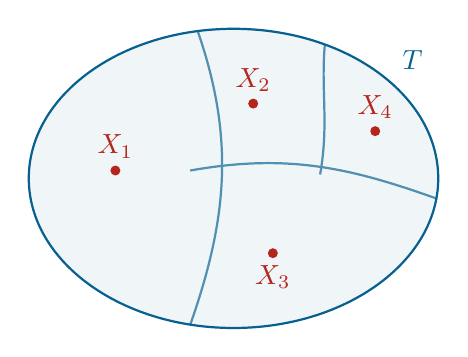
\begin{tikzpicture}
    % (1) Fill of T
    \fill[figBlue!6] (0, 0) ellipse (2.6 and 1.9);

    % (2) Orbit partition lines clipped to T
    \begin{scope}
        \clip (0, 0) ellipse (2.6 and 1.9);
        \draw[thick, figBlue!70] (-0.6, -2.0) to[out=70, in=-70] (-0.5, 2.0);
        \draw[thick, figBlue!70] (-0.55, 0.1) to[out=10, in=160] (2.7, -0.3);
        \draw[thick, figBlue!70] (1.1, 0.05) to[out=80, in=-100] (1.2, 2.0);
    \end{scope}

    % (3) Outer boundary of T
    \draw[thick, figBlue] (0, 0) ellipse (2.6 and 1.9);

    % (4) Orbit representatives
    \fill[figRed] (-1.5, 0.1) circle (1.8pt)
                  (0.25, 0.95) circle (1.8pt)
                  (0.5, -0.95) circle (1.8pt)
                  (1.8, 0.6) circle (1.8pt);

    % (5) Text last
    \node[anchor=south west, inner sep=0.15cm, figBlue] at (1.99, 1.22) {$T$};
    \node[anchor=south, inner sep=0.15cm, figRed] at (-1.5, 0.1) {$X_1$};
    \node[anchor=south, inner sep=0.15cm, figRed] at (0.25, 0.95) {$X_2$};
    \node[anchor=north, inner sep=0.15cm, figRed] at (0.5, -0.95) {$X_3$};
    \node[anchor=south, inner sep=0.15cm, figRed] at (1.8, 0.6) {$X_4$};
\end{tikzpicture}
\end{center}
\end{content}

\begin{speech}[00:12:49 - 00:14:00]
Now, the left-hand side, this is $n$ choose $p$ to the $k$, okay \inlinemetanote{writes $\binom{n}{p^k}$ below $|T|$}? And what we know about this is $p$ does not divide this \inlinemetanote{writes: $p \nmid |T|$}. That's where we started. That means that $p$ cannot divide every orbit.

So, the conclusion here is: there must exist some orbit --- there must exist some $X_i$ --- such that $p$ does not divide the size of that orbit \inlinemetanote{writes: So $\exists \, X_i$ such that $p \nmid |\operatorname{Orb}(X_i)|$}, okay? Because if it divided all of them, it'd divide this, but it can't divide that.

We're going to look at that one, this $X_i$. Maybe I should call it $X_j$, because there exists some $X_j$ \inlinemetanote{changes $X_i$ to $X_j$} --- that's the $j$ letter --- there's some very special $X_j$ such that $p$ does not divide the orbit size.
\end{speech}

\begin{content}[Existence of an Orbit Not Divisible by \texorpdfstring{$p$}{p}]
Using \eqref{eq:cardinality-T}, \eqref{eq:p-not-div-binom}, and \eqref{eq:orbit-decomp-T}, we have:
\[
|T| = \binom{n}{p^k} = \sum_{X_i} |\operatorname{Orb}(X_i)|, \qquad \text{with } p \nmid |T|.
\]
If $p$ divided $|\operatorname{Orb}(X_i)|$ for every orbit representative $X_i$, then $p$ would divide the sum $|T|$, contradicting $p \nmid |T|$. Therefore, there exists at least one distinguished representative $X_j \in T$ (renaming the index from $i$ to $j$) such that:
\begin{equation}\label{eq:orbit-xj-coprime}
p \nmid |\operatorname{Orb}(X_j)|.
\end{equation}
\end{content}

\begin{speech}[00:14:00 - 00:15:50]
All right, so now we use the Orbit--Stabilizer Theorem for that orbit \inlinemetanote{wipes a spot on the lower-right board and writes: Use Orb-Stab Thm}. So, use this Orbit--Stabilizer Theorem, and what does it say? It says the size of $G$ divided by the size of the stabilizer of that $X_j$ equals the size of this orbit \inlinemetanote{writes: $\frac{|G|}{|\operatorname{Stab}(X_j)|} = |\operatorname{Orb}(X_j)|$}. That's the Orbit--Stabilizer Theorem.

Okay, and what do we know? That this thing here --- the size of $G$ --- is $n$, and $n$ is equal to $p$ to the $k$ times $m$, okay \inlinemetanote{writes $p^k m$ with an arrow to $|G|$}? That's what the top is here, right?

And this thing has no $p$'s, because $p$ does not divide this, okay \inlinemetanote{writes \qt{has no $p$'s} with an arrow to $|\operatorname{Orb}(X_j)|$}? So, where could all the $p$'s go? How can you have this? We've got a lot of $p$'s here, no $p$'s here. How could this happen?

All the $p$'s have to be here \inlinemetanote{points at $|\operatorname{Stab}(X_j)|$}. They have to kill all the $p$'s. So, the conclusion here is that $p$ to the $k$ divides the stabilizer --- well, the size of the stabilizer \inlinemetanote{writes: $\implies p^k \mid |\operatorname{Stab}(X_j)|$}. Because there's conservation of $p$'s, they can't just leave.

Okay, is that clear? We got a big number of $p$'s here, $p$ to the $k$, and there's no $p$'s here. The only way to get rid of them is if we had divided them out, okay?
\end{speech}

\begin{content}[Applying the Orbit--Stabilizer Theorem]
Applying the Orbit--Stabilizer Theorem to the distinguished element $X_j \in T$ gives:
\[
\frac{\overbrace{|G|}^{p^k m}}{|\operatorname{Stab}(X_j)|} = \underbrace{|\operatorname{Orb}(X_j)|}_{\text{has no } p\text{'s}}.
\]
Cross-multiplying, we have $p^k m = |\operatorname{Stab}(X_j)| \cdot |\operatorname{Orb}(X_j)|$. Since $p$ is prime and $p \nmid |\operatorname{Orb}(X_j)|$ by \eqref{eq:orbit-xj-coprime}, Euclid's lemma (unique prime factorization) forces all $k$ factors of $p$ in $p^k m$ to divide $|\operatorname{Stab}(X_j)|$:
\begin{equation}\label{eq:pk-divides-stab}
p^k \mid |\operatorname{Stab}(X_j)|.
\end{equation}
\end{content}

\begin{speech}[00:15:50 - 00:16:33]
And so this proves, for this special one --- for this very special $X_j$ \inlinemetanote{writes: for $X_j$} --- the order of the stabilizer is... I'm never going to do this again \inlinemetanote{discards a chalk stick}. It is at least $p$ to the $k$, otherwise how could it divide it \inlinemetanote{writes: $|\operatorname{Stab}(X_j)| \ge p^k$}? It's not zero.

Okay, and that's it. That's like an amazingly gorgeous proof. So, we found the group now: it's the stabilizer of this particular one. It has size less than $p$ to the $k$ and greater than $p$ to the $k$, so it has size $p$ to the $k$ and we're done \inlinemetanote{writes boxed $|\operatorname{Stab}(X_j)| = p^k$ and draws a QED square}. So, that is an amazing proof. \inlinemetanote{pushes the bottom board up}
\end{speech}

\begin{content}[Conclusion of the Proof]
For $X_j \in T$, since $|\operatorname{Stab}(X_j)|$ is a positive integer divisible by $p^k$ by \eqref{eq:pk-divides-stab}, it satisfies:
\[
|\operatorname{Stab}(X_j)| \ge p^k.
\]
Combining this lower bound with \cref{lem:stab-upper-bound} ($|\operatorname{Stab}(X_j)| \le p^k$) yields:
\[
\boxed{|\operatorname{Stab}(X_j)| = p^k.}
\]
Thus, $S := \operatorname{Stab}(X_j) \subset G$ is the desired subgroup of order $p^k$, completing the proof of \cref{thm:sylow-1}.

\begin{steps}[Summary of the Proof Strategy]
The existence of a subgroup of order $p^k$ is obtained by sandwiching the order of $\operatorname{Stab}(X_j)$ from both sides:
\begin{enumerate}[label=\textbf{\arabic*.}]
    \item \textbf{Upper bound (for every $X \in T$):} Left translation of a single fixed element $a_1 \in X$ yields an injection $\operatorname{Stab}(X) \hookrightarrow X$, so $|\operatorname{Stab}(X)| \le |X| = p^k$.
    \item \textbf{Lower bound (for a special $X_j \in T$):} Because $p \nmid |T| = \binom{n}{p^k}$, at least one orbit $\operatorname{Orb}(X_j)$ has size coprime to $p$. By the Orbit--Stabilizer Theorem, $p^k \mid |\operatorname{Stab}(X_j)|$, so $|\operatorname{Stab}(X_j)| \ge p^k$.
\end{enumerate}
Hence, $|\operatorname{Stab}(X_j)| = p^k$, and the stabilizer subgroup $\operatorname{Stab}(X_j)$ itself is the subgroup $S$ required by Sylow I.
\end{steps}
\end{content}

\end{proofWrapper}

\begin{speech}[00:16:33 - 00:17:03]
\inlinemetanote{pushes the lower board up} So, this is a proof that shows the power of thinking about these group actions, but it's a really amazing proof.

Okay, that's Sylow $1$, that we have one of the subgroups now. \inlinemetanote{pushes the lower-left board up}
\end{speech}

\begin{hidden}
% timestamp: 00:04:13
% topic: Proof of Sylow I completed; transitioning to Sylow's Second Theorem
% board_state: thm:sylow-1, lem:stab-upper-bound, eq:p2-pk-divides-stab
% next_goal: State Sylow II, define p-Sylow subgroup, and begin proof of Sylow II
% open_loops: none
\end{hidden}

\section{Sylow's Second Theorem}

\begin{speech}[00:17:03 - 00:18:39]
Okay, so Sylow $2$ says something else. So, we're going to state Sylow $2$ \inlinemetanote{writes: Sylow II}. It's the same hypotheses. I don't write them again: we have $G$ is a group of order $n$, and we have $p$ to the $k$ is the biggest power of $p$ that divides $n$. Maybe I write it anyway, so we don't get confused \inlinemetanote{writes \qt{Let $H \subset G$} and \qt{$|G| = n = m \cdot p^k$, $(p, m) = 1$}}.

So, let $H$ be any subgroup of order $p$ to the $\ell$, okay \inlinemetanote{writes \qt{be any subgroup} and \qt{of order $p^\ell$}}? So, we just take any subgroup of order $p$ to the $\ell$. Of course, in this case, $\ell$ has to be less than or equal to $k$ by Lagrange \inlinemetanote{writes: ($\ell \le k$ by Lagrange)}. Because a subgroup has to have an order which divides. So, we take any one.

Then Sylow $2$ says that $H$ lies in a subgroup $S$... Let me write it as \qt{there exists}: there exists $S$ in $G$ such that $H$ is in $S$ and the order of $S$ is $p$ to the $k$ \inlinemetanote{writes boxed \qt{$\exists \, S \subset G$ such that $H \subset S$, $|S| = p^k$}}. So, this says that if you take any subgroup of order $p$ to the $\ell$, actually it sits inside one of our subgroups of order $p$ to the $k$.
\end{speech}

\begin{content}
\begin{theorem}[Sylow II]\label[theorem]{thm:sylow-2}
Let $G$ be a finite group with $|G| = n = m \cdot p^k$, where $p$ is prime and $(p, m) = 1$. Let $H \subset G$ be any subgroup of order $p^\ell$ (note that $\ell \le k$ by Lagrange's Theorem, since $|H| \mid |G|$ and $(p, m) = 1$). Then:
\[
\boxed{\exists \, S \subset G \quad \text{such that} \quad H \subset S, \; |S| = p^k.}
\]
\end{theorem}
\end{content}

\begin{speech}[00:18:39 - 00:19:58]
So, the terminology for this, by the way, is that for $G$, if $S$ is a subgroup of $G$ where $S$ is of order $p$ to the $k$, then this is the definition: $S$ is called a \newterm{$p$-Sylow subgroup} \inlinemetanote{writes \qt{For $S \subset G$, $|S| = p^k$} and boxed \qt{$S$ is called a $p$-Sylow subgroup}}.

If you have a finite group, and you take this maximal power of $p$, if you ever find a subgroup of that order, it's called a $p$-Sylow subgroup. Sylow $1$ says there exist $p$-Sylow subgroups. Sylow $2$ says that if I take any subgroup of order $p$ to the $\ell$, it actually sits inside a $p$-Sylow subgroup, okay?

So, maybe I write that in words: Sylow $2$ says that every subgroup $H$ in $G$, where $H$ has some power of $p$ order, sits in a $p$-Sylow subgroup \inlinemetanote{writes: Sylow II: every subgroup $H \subset G$ with $|H| = p^\ell$, $H$ sits in a $p$-Sylow subgroup}. I'm just saying over what I've said already. So, we have to prove it.
\end{speech}

\begin{content}[Terminology and Reformulation of Sylow II]
\begin{definition}[$p$-Sylow Subgroup]\label[definition]{def:p-sylow-subgroup}
Let $G$ be a finite group of order $|G| = n = m \cdot p^k$ with $(p, m) = 1$. A subgroup $S \subset G$ with $|S| = p^k$ (the highest power of $p$ dividing $|G|$) is called a \newterm{$p$-Sylow subgroup} of $G$.
\end{definition}

\begin{remark}[Reformulation of Sylow I and Sylow II]\label[remark]{rem:sylow-1-2-terminology}
In this terminology, Sylow I (\cref{thm:sylow-1}) asserts that $p$-Sylow subgroups of $G$ exist, and Sylow II (\cref{thm:sylow-2}) states that every subgroup $H \subset G$ whose order is a power of $p$ ($|H| = p^\ell$) is contained in some $p$-Sylow subgroup of $G$ ($H \subset S$).
\end{remark}
\end{content}

\begin{proofWrapper}[Proof of \cref{thm:sylow-2}]

\subsection{Setup and Reduction to \texorpdfstring{$\ell > 0$}{l > 0}}

\begin{speech}[00:19:58 - 00:21:10]
All right, so we have to name one, so let's call it $P$. I'm going to give the proof now \inlinemetanote{writes: Proof.}.

So, let $P$ in $G$ be a $p$-Sylow subgroup \inlinemetanote{writes: Let $P \subset G$ be a $p$-Sylow subgp.}. The size of this is $p$ to the $k$ \inlinemetanote{writes: $|P| = p^k$}. It's capital $P$. This exists by Sylow $1$ \inlinemetanote{writes: (Sylow I)}.

And now we have $H$: we are given a subgroup $H$ in $G$ where the order of $H$ is $p$ to the $\ell$ \inlinemetanote{writes: We are given $H \subset G$, $|H| = p^\ell$}. And first of all, we can just assume $\ell$ is positive \inlinemetanote{writes: $\ell > 0$}, because if we were given a subgroup of order $p$ to the zero, that subgroup is order $1$, which means it's only the neutral element, and the neutral element sits inside here (i.e., inside $P$), so we don't have to confuse ourselves with this case. So, we can assume that $\ell$ is positive.

Okay, and we're going to use a group action, of course. \inlinemetanote{pushes the lower-right board up}
\end{speech}

\begin{content}[Choice of \texorpdfstring{$P$}{P} and Reduction to \texorpdfstring{$\ell > 0$}{l > 0}]
Let $P \subset G$ be a $p$-Sylow subgroup, so that $|P| = p^k$; such a subgroup exists by Sylow I (\cref{thm:sylow-1}).

We are given a subgroup $H \subset G$ of order $|H| = p^\ell$. We may assume $\ell > 0$: if $\ell = 0$, then $|H| = p^0 = 1$, so $H = \{e\}$ consists solely of the identity element, which automatically lies in $P$ (since $P$ is a subgroup of $G$).
\end{content}

\begin{hidden}
% timestamp: 00:08:20
% topic: Proof of Sylow II -- setup of P and H, reduction to l > 0
% board_state: thm:sylow-2, def:p-sylow-subgroup, rem:sylow-1-2-terminology
% next_goal: Define restricted left coset action H \curvearrowright G/P and find an H-fixed point
% open_loops: none
\end{hidden}

\subsection{Restricting the Left Coset Action to \texorpdfstring{$H$}{H}}

\begin{speech}[00:21:10 - 00:22:43]
So, the question is: which group action do we use for this \inlinemetanote{erases the lower-left board}?

We have $G$ and our $p$-Sylow subgroup $P$ \inlinemetanote{writes: $P \subset G$}, so we can consider this coset space: this is the set of left cosets \inlinemetanote{writes: $\frac{G}{P}$ set of left cosets}. And we have seen that $G$ acts on this \inlinemetanote{writes: $G \curvearrowright \frac{G}{P}$}. That's the standard action on left cosets \inlinemetanote{writes \qt{standard action on left cosets} with an arrow to $\curvearrowright$}. We discussed this yesterday.

Okay, but that's not $H$, there's no $H$ there. But we can always act by a subgroup here. So, this is the standard action, and we can just restrict this to inside $H$, so we get $H$ cross $G$ mod $P$ to $G$ mod $P$, okay \inlinemetanote{writes \qt{$G \times \frac{G}{P} \to \frac{G}{P}$}, $\cup$ below $G$, and \qt{$H \times \frac{G}{P} \to \frac{G}{P}$}}?

So, this is the action we're going to take. Is this restriction clear? We already know how $G$ acts on left cosets. $H$ is a subgroup, so it just acts as if it were an element of $G$. Okay, so this is the action we'll consider: we consider this action in the proof \inlinemetanote{writes \qt{We consider this action} with an arrow to $H \times \frac{G}{P} \to \frac{G}{P}$}.
\end{speech}

\begin{content}[The Restricted Action \texorpdfstring{$H \curvearrowright \frac{G}{P}$}{H acts on G/P}]
Given $P \subset G$, let $\frac{G}{P} := \{ g P \mid g \in G \}$ be the set of left cosets of $P$ in $G$. Recall the standard left-multiplication action of $G$ on $\frac{G}{P}$:
\[
G \curvearrowright \frac{G}{P}, \qquad g \cdot (x P) := (g x) P.
\]
Since $H \subset G$ is a subgroup, we restrict this standard action from $G$ to $H$:
\[
\begin{array}{c@{}c@{}c@{}l}
G & \times & \dfrac{G}{P} & \longrightarrow \dfrac{G}{P} \\[6pt]
\cup & & & \\[4pt]
H & \times & \dfrac{G}{P} & \longrightarrow \dfrac{G}{P}
\end{array}
\]
given by $h \cdot (x P) := (h x) P$ for $h \in H$ and $x P \in \frac{G}{P}$. We analyze this restricted action $H \curvearrowright \frac{G}{P}$ in the remainder of the proof.
\end{content}

\begin{aiNote}[Notation: \texorpdfstring{$\frac{G}{P}$}{G/P} for the Set of Left Cosets]
% [PERSISTENT]
On the board, the lecturer writes the set of left cosets of $P$ in $G$ vertically with a horizontal bar as $\frac{G}{P}$ (pronouncing it \qt{$G$ mod $P$}) rather than inline $G/P$, because $P$ is not assumed normal and the cardinality $|\frac{G}{P}|$ equals $\frac{|G|}{|P|}$. We preserve $\frac{G}{P}$ throughout.
\end{aiNote}

\begin{speech}[00:22:43 - 00:23:47]
Okay, so what are we going to do with this action? I'll try to make big $P$'s here so you don't get confused. What are we going to do with this action? Well, we'd like to know what is the size of this set \inlinemetanote{writes: $\left|\frac{G}{P}\right|$}. And the answer is that we know this is $n$, and this is $p$ to the $k$, and so this is $m$ \inlinemetanote{writes: $= \frac{n}{p^k} = m$}. Because Lagrange says that the size of this is equal to the size of $G$, size of $P$ \inlinemetanote{writes $\frac{|G|}{|P|}$ below $\left|\frac{G}{P}\right|$}, okay?

So, that's $m$. And we know one thing about $m$: $p$ does not divide $m$ \inlinemetanote{writes: $p \nmid m$}. All right?

This means we have $H$ acting on this $G$ mod $P$, and the size of this set here is not divisible by $p$ \inlinemetanote{writes \qt{$H \curvearrowright \frac{G}{P}$} and \qt{$\left|\frac{G}{P}\right|$ is not div. by $p$}}.
\end{speech}

\begin{content}[Cardinality of \texorpdfstring{$\frac{G}{P}$}{G/P} and Non-Divisibility by \texorpdfstring{$p$}{p}]
By Lagrange's Theorem, the number of left cosets of $P$ in $G$ is:
\[
\left|\frac{G}{P}\right| = \frac{|G|}{|P|} = \frac{n}{p^k} = m.
\]
Since $(p, m) = 1$, we have $p \nmid m$. Consequently, for the action $H \curvearrowright \frac{G}{P}$, the set $\frac{G}{P}$ has cardinality not divisible by $p$:
\begin{equation}\label{eq:p2-gp-not-div-p}
p \nmid \left|\frac{G}{P}\right|.
\end{equation}
\end{content}

\subsection{Existence of an \texorpdfstring{$H$}{H}-Fixed Point in \texorpdfstring{$\frac{G}{P}$}{G/P}}

\begin{speech}[00:23:47 - 00:25:07]
All right. So, the conclusion --- and we've seen this kind of argument before --- the conclusion we will see is that there must be a fixed point, an $H$-fixed point in $G$ mod $P$, all right \inlinemetanote{writes: Conclusion is that there must be an $H$-fixed pt in $\frac{G}{P}$}?

I'll give you an argument for this, but it should not be a surprise. Well, I'll say it in words and I'll write it down clear, because we can divide this \inlinemetanote{points at $\frac{G}{P}$} in terms of the orbits, right? And the orbits always have orders that are divisible by the order of $H$. That's by the Orbit--Stabilizer Theorem.

This (i.e., $|H|$) is a power of $p$. So, the only possibility for the orbits are powers of $p$. If all the orbits took positive powers of $p$, then this (i.e., $\left|\frac{G}{P}\right|$) would be divisible by $p$. But it's not divisible by $p$. So, there must be one orbit that takes the only power of $p$ that's not divisible by $p$, which is $p$ to the zero, and that would be a fixed point. That's the argument in words, we can write it. But we've done this argument before. \inlinemetanote{pushes the lower-left board up}
\end{speech}

\begin{content}[Fixed-Point Claim]
\begin{claim}[Existence of an $H$-Fixed Point in $\frac{G}{P}$]\label[claim]{clm:h-fixed-point-gp}
Under the action $H \curvearrowright \frac{G}{P}$, there exists an $H$-fixed point in $\frac{G}{P}$ (i.e., an orbit of size $1 = p^0$).
\end{claim}
\end{content}

\begin{aiNote}[Slip of the Tongue: \qt{orders that are divisible by the order of $H$}]
% [PERSISTENT]
In the preceding explanation, the lecturer says that the orbits \qt{have orders that are divisible by the order of $H$}. By the Orbit--Stabilizer Theorem, $|\operatorname{Orb}(z)| = \frac{|H|}{|\operatorname{Stab}(z)|}$, so the size of each orbit \emph{divides} the order of $H$ (rather than being divisible by $|H|$). Since $|H| = p^\ell$ is a power of $p$, every divisor of $|H|$ is itself a power of $p$, as the lecturer states immediately afterward.
\end{aiNote}

\begin{speech}[00:25:14 - 00:27:23]
What's important in this argument is the size of $H$ is a power of $p$, and the size of the set does not divide $p$... $p$ is not divisible by that, sorry. $p$ does not divide the size of the set \inlinemetanote{erases the lower-right board}.

So, let's try to write it out somehow longhand. The picture that we've drawn many times now: here $H$ is acting on this set, this is cosets here \inlinemetanote{draws a closed contour labeled $\frac{G}{P}$ with $H \curvearrowright$}. So, this breaks up into the orbit spaces, okay \inlinemetanote{partitions $\frac{G}{P}$ into orbit regions}?

And the Orbit--Stabilizer Theorem says --- I mean, sorry, the size here, this is equal to $m$, is equal to the sum of all the orbits. It's the same thing we always write. So, maybe I put $z_i$ here \inlinemetanote{writes: $m = \left|\frac{G}{P}\right| = \sum_{z_i} |\operatorname{Orb}(z_i)|$}. We have some $z_1$ here, and $z_2$ here, and so on, okay \inlinemetanote{marks points $z_1, z_2$ inside the orbit regions}? This is what we always write.

Now, the Orbit--Stabilizer Theorem says that the size of this orbit is equal to the size of $H$ divided by the size of the stabilizer, okay \inlinemetanote{writes: $|\operatorname{Orb}(z_i)| = \frac{|H|}{|\operatorname{Stab}(z_i)|}$}? This thing, $H$ upstairs, is a power of $p$ --- that's all it is, there's nothing else. The order of $H$ is a power of $p$, that was the assumption \inlinemetanote{writes $p^\ell$ above $|H|$}. So, the only possibilities for this orbit are powers of $p$. That's it.

But it cannot be that every orbit is a positive power of $p$, because then this thing (i.e., $m$) would be divisible by $p$, and it's not divisible by $p$, because $m$ is not divisible by $p$. So, there must be one orbit whose size is not a positive power of $p$. It has to be a power of $p$, but not a positive power of $p$. So, the only possibility is $p$ to the zero, and that orbit is a fixed point.
\end{speech}

\begin{content}[Orbit Decomposition of \texorpdfstring{$\frac{G}{P}$}{G/P} and Orbit--Stabilizer Proof]
\begin{proof}[Proof of \cref{clm:h-fixed-point-gp}]
Decomposing $\frac{G}{P}$ into its disjoint $H$-orbits and choosing a representative $z_i \in \frac{G}{P}$ from each orbit, we obtain:
\begin{equation}\label{eq:p2-gp-orbit-sum}
m = \left|\frac{G}{P}\right| = \sum_{z_i} |\operatorname{Orb}(z_i)|.
\end{equation}

\definecolor{figBlue}{HTML}{07608F} % RGB (7, 96, 143): petrol blue (MidnightBlue)
\definecolor{figRed}{HTML}{B5251C} % RGB (181, 37, 28): brick red (BrickRed)
\begin{hidden}
- Canvas: no scale, cm; ellipse G/P centred at (0, 0) with radii 2.6 and 1.9; picture spans x in [-3.1, 3.0], y in [-2.0, 2.2].
- Order: (1) light fill of G/P; (2) orbit partition curves clipped inside the ellipse; (3) outer outline of G/P;
  (4) representative dots z_1 and z_2; (5) all text last.
- Partition curves (clipped inside ellipse 2.6 x 1.9):
  Curve 1 (top cell boundary): (-2.7, 0.65) to[out=-15, in=195] (2.7, 0.65);
  Curve 2 (middle split): (-2.7, -0.4) to[out=10, in=170] (2.7, -0.35);
  Curve 3 (vertical split across lower cells): (-0.2, 0.62) to[out=-85, in=95] (0.1, -1.95).
- Representative dots, well inside their cells:
  z_1 = (0.0, 1.25) in the top cell (0.60 above curve 1, 0.65 below the ellipse top 1.9);
  z_2 = (-1.25, 0.12) in the middle-left cell (between y = -0.35 and 0.62, and 1.05 left of curve 3).
- Labels (attached with inner sep=0.15cm):
  "H \curvearrowright" anchor=south east at (-1.95, 1.40) (outside the upper-left outline at 135 deg, (-1.84, 1.34));
  "\frac{G}{P}" anchor=south west at (1.99, 1.22) (outside the upper-right outline at 40 deg);
  "z_1" anchor=west at (0.0, 1.25) (right of dot, inside top cell where ellipse reaches x = 1.96);
  "z_2" anchor=west at (-1.25, 0.12) (right of dot, clear of curve 3 at x ~ -0.15).
- Collisions: both exterior labels sit outside the ellipse on opposite sides; z_1 and z_2 stay inside their own orbit cells
  at least 0.4 cm from every partition curve.
\end{hidden}
\begin{center}
\begin{tikzpicture}
    % (1) Fill of G/P
    \fill[figBlue!6] (0, 0) ellipse (2.6 and 1.9);

    % (2) Orbit partition curves clipped inside G/P
    \begin{scope}
        \clip (0, 0) ellipse (2.6 and 1.9);
        \draw[thick, figBlue!70] (-2.7, 0.65) to[out=-15, in=195] (2.7, 0.65);
        \draw[thick, figBlue!70] (-2.7, -0.4) to[out=10, in=170] (2.7, -0.35);
        \draw[thick, figBlue!70] (-0.2, 0.62) to[out=-85, in=95] (0.1, -1.95);
    \end{scope}

    % (3) Outer boundary of G/P
    \draw[thick, figBlue] (0, 0) ellipse (2.6 and 1.9);

    % (4) Orbit representatives
    \fill[figRed] (0.0, 1.25) circle (1.8pt) (-1.25, 0.12) circle (1.8pt);

    % (5) Text last
    \node[anchor=south east, inner sep=0.15cm] at (-1.95, 1.40) {$H \curvearrowright$};
    \node[anchor=south west, inner sep=0.15cm, figBlue] at (1.99, 1.22) {$\dfrac{G}{P}$};
    \node[anchor=west, inner sep=0.15cm, figRed] at (0.0, 1.25) {$z_1$};
    \node[anchor=west, inner sep=0.15cm, figRed] at (-1.25, 0.12) {$z_2$};
\end{tikzpicture}
\end{center}

By the Orbit--Stabilizer Theorem applied to the action of $H$, the size of each orbit is:
\[
|\operatorname{Orb}(z_i)| = \frac{\overbrace{|H|}^{p^\ell}}{|\operatorname{Stab}(z_i)|}.
\]
Because $|H| = p^\ell$ is a power of the prime $p$, every divisor of $|H|$ is also a power of $p$. Thus, $|\operatorname{Orb}(z_i)| = p^{r_i}$ for some integer $r_i$ with $0 \le r_i \le \ell$.

If every orbit had size $p^{r_i}$ with $r_i \ge 1$ (a positive power of $p$), then $p$ would divide every term in \eqref{eq:p2-gp-orbit-sum}, implying $p \mid m = \left|\frac{G}{P}\right|$, which contradicts \eqref{eq:p2-gp-not-div-p}. Therefore, at least one orbit must have size not divisible by $p$, so $r_i = 0$ and $|\operatorname{Orb}(z_i)| = p^0 = 1$. That representative $z_i$ is an $H$-fixed point in $\frac{G}{P}$.
\end{proof}
\end{content}

\begin{hidden}
% timestamp: 00:14:33
% topic: Proof of H-fixed point in G/P completed; expressing fixed point as coset xP
% board_state: thm:sylow-2, clm:h-fixed-point-gp, eq:p2-gp-not-div-p, eq:p2-gp-orbit-sum
% next_goal: Write the fixed point z_i as a left coset x P and derive h x P = x P for all h \in H
% open_loops: none
\end{hidden}

\begin{speech}[00:27:23 - 00:29:23]
So, there exists $z_i$ such that $\operatorname{Orb}(z_i)$ is equal to $p$ to the zero, and then $z_i$ is an $H$-fixed point \inlinemetanote{writes: $\exists \, z_i \text{ s.t. } |\operatorname{Orb}(z_i)| = p^0$, $\text{then } z_i \text{ is } H\text{-fixed pt.}$}, because it means that the stabilizer takes up all of $H$, and it's a fixed point.

All right, so we found one $z_i$. This $z_i$, this one that's a fixed point, is an element of this \inlinemetanote{writes: $z_i \in \frac{G}{P}$}, right? So, it's a coset space, so we can write $z_i$ as some $x P$ \inlinemetanote{writes: $z_i = x P$}. That's the left coset of $x$, where $x$ is in $G$ \inlinemetanote{writes: $x \in G$}. So, this $z_i$ is an element of this coset space, and now I'm just writing it explicitly as a coset.

And what we know about this is it's a fixed point. That means we know, since it's an $H$-fixed point... I don't have to say $H$-fixed, I could just say fixed for the action we're considering, but since there's $G$'s and $H$'s, I'm just being very specific and saying $H$-fixed point. It's an $H$-fixed point. We know that if I take any element in $H$, if I take $h x$, this coset, it has to be just this coset, okay \inlinemetanote{writes \qt{We know (H-fixed pt.)} and \qt{$\forall h$, $h x P = x P$}}? That's what it means, for any $h$.

All right, so we're going to look at this equation: what does it say \inlinemetanote{pushes the lower-right board up}? But the whole point of this analysis of this action of $H$ on the left coset space was to find this fixed point. That was the whole purpose of that analysis. Well, we found it now, and that fixed point has this property. \inlinemetanote{erases the lower-left board}
\end{speech}

\begin{content}[The Fixed Coset and Its Invariance Equation]
By \cref{clm:h-fixed-point-gp}, there exists $z_i \in \frac{G}{P}$ such that $|\operatorname{Orb}(z_i)| = p^0 = 1$, meaning $z_i$ is an $H$-fixed point. Writing $z_i$ explicitly as a left coset of $P$ in $G$, we have:
\[
z_i = x P \qquad \text{for some } x \in G.
\]
Since $z_i$ is an $H$-fixed point under the left-multiplication action of $H$ on $\frac{G}{P}$, every element $h \in H$ leaves $x P$ invariant:
\begin{equation}\label{eq:p2-fixed-coset}
\forall h \in H, \qquad h x P = x P.
\end{equation}
\end{content}

\subsection{Concluding the Containment from the Fixed-Point Equation}

\begin{speech}[00:29:24 - 00:30:35]
So, let's try to think about this fixed-point equation. We remember here that $P$ inside $G$, to start, was a $p$-Sylow subgroup \inlinemetanote{writes: $P \subset G$ is $p$-Sylow subgp.}. So, in particular, the order of this is $p$ to the $k$ \inlinemetanote{writes: $|P| = p^k$}.

And now we have the fixed-point equation \inlinemetanote{writes: Fixed point equation}. The fixed-point equation says --- I just repeat it --- for every $h$, if I take $h$ times this coset, I get back this coset \inlinemetanote{writes: $\forall h \in H$, $h x P = x P$}. All right, so I write here: $x P$ in $\frac{G}{P}$ is $H$-fixed \inlinemetanote{writes: $x P \in \frac{G}{P}$ is $H$-fixed}.

So, this is the summary from the previous part. We start with this $p$-Sylow subgroup. It has the right order for the maximum power of $p$. There's the $H$-action. By our analysis of this Orbit--Stabilizer Theorem, there is some coset here which is $H$-fixed. This is the $H$-fixed equation, and that's for every $h$ --- oh, it's already written there \inlinemetanote{writes \qt{$\forall h$} at the bottom left and points at $\forall h \in H$ above}.
\end{speech}

\begin{content}[Summary of the Fixed-Point Setup]
Summarizing the ingredients obtained so far:
\begin{itemize}
    \item $P \subset G$ is a $p$-Sylow subgroup, so $|P| = p^k$.
    \item $x P \in \frac{G}{P}$ is an $H$-fixed point, satisfying the fixed-point equation:
    \[
    \forall h \in H, \qquad h x P = x P.
    \]
\end{itemize}
\end{content}

\begin{speech}[00:30:35 - 00:32:09]
Okay, so we need to think a little bit about what this means. When I write this \inlinemetanote{writes: $h x P$}, I hope you understand what this coset is, you know: $x$ is an element of $G$, $h$ is an element of $H$ inside $G$, so when I multiply $h$ times $x$, that's inside $G$, and this is the coset \inlinemetanote{writes \qt{$x \in G$} and \qt{$h \in H \subset G$}}.

All right? So, in particular, $h x$ is in this coset, because in this $P$ you could put $1$ there \inlinemetanote{writes \qt{$h x P \ni h x$} and \qt{$h x \in h x P$}}. But it better be also in this coset. So, that means $h x$ must also be here, in $x P$ \inlinemetanote{writes: $h x$ must also be in $x P$}.

What does that mean? That means that there must be some element $z$ in $P$ such that $h x$ equals $x z$, where this is an element of $P$, this is an element of $G$, this is an element of $G$ --- that's the fixed one \inlinemetanote{writes \qt{$\exists \, z \in P$ such that $h x = x z$} and \qt{$\in P$} below $z$}. We're not ever moving $x$, $x$ is already chosen here. So, these are some fixed... maybe I should erase it, because I don't have... $x$ is fixed. We start with $h$, $x$ is fixed, then we can always solve --- it's saying we can always solve this equation.

I mean, we found our $x$, and it says that for every $h$, we can solve this equation: that $h x$ equals $x$ times something in $P$, we can always solve it. That's what it says.
\end{speech}

\begin{content}[Coset Membership and the Equation \texorpdfstring{$h x = x z$}{h x = x z}]
Let $h \in H \subset G$ and $x \in G$. Since $P$ is a subgroup, it contains the identity element $e \in P$ (written $1$ in multiplicative notation), and thus the coset $h x P$ contains $h x \cdot 1 = h x$:
\[
h x P \ni h x \qquad (\text{i.e., } h x \in h x P).
\]
By the fixed-point equation \eqref{eq:p2-fixed-coset}, $h x P = x P$, so $h x$ must also belong to $x P$. By the definition of the left coset $x P = \{ x z \mid z \in P \}$, there exists an element $z \in P$ such that:
\begin{equation}\label{eq:p3-hx-xz}
h x = x z.
\end{equation}
\end{content}

\begin{hidden}
% timestamp: 00:06:29
% topic: Proof of Sylow II -- rewriting h x P = x P as h x = x z with z in P
% board_state: thm:sylow-2, eq:p3-fixed-coset, eq:p3-hx-xz
% next_goal: Solve for h = x z x^{-1}, conclude H \subset x P x^{-1}, finish Sylow II, and state/prove Sylow III
% open_loops: none
\end{hidden}

\begin{speech}[00:32:09 - 00:33:27]
So, what does that mean? That means that actually $h$ is equal to $x z x$ inverse \inlinemetanote{writes: $h = x z x^{-1}$}. And if I rewrite this, this means that $h$ is in the conjugation of $P$ \inlinemetanote{writes: $h \in x P x^{-1}$}.

Remember conjugation: conjugation is a group automorphism. So, if $P$ is a subgroup of $G$, then $x P x$ inverse is also a subgroup of $G$ \inlinemetanote{writes \qt{$P \subset G$} and \qt{$x P x^{-1}$}}. It may be a different subgroup, maybe not, but anyway, it's a subgroup of $G$. And it's also a $p$-Sylow subgroup. The order of this is the same as the order of $P$, because conjugation is a bijective operation \inlinemetanote{writes \qt{$|x P x^{-1}|$} and \qt{$= |P|$}}. And the order is $p$ to the $k$ \inlinemetanote{writes: $= p^k$}.

And this is for any $h$. That means $H$ is inside $x P x$ inverse, and then we're done \inlinemetanote{writes \qt{$H \subset x P x^{-1}$} and draws a QED square}. Because this is a conjugate of the subgroup $P$ that we started with. Such a conjugate has the same order as $P$, so in particular the conjugate's also a $p$-Sylow subgroup, and we were trying to find a $p$-Sylow subgroup that contains $H$, and we found it. So, that's the end of the proof.
\end{speech}

\begin{content}[Conjugation of \texorpdfstring{$P$}{P} and Containment of \texorpdfstring{$H$}{H}]
Multiplying \eqref{eq:p3-hx-xz} on the right by $x^{-1}$ in $G$ gives:
\[
h = x z x^{-1}.
\]
Since $z \in P$, this means $h \in x P x^{-1}$.

Because conjugation by $x \in G$ (namely, the map $g \mapsto x g x^{-1}$) is a group automorphism of $G$, it maps the subgroup $P \subset G$ to a subgroup $x P x^{-1} \subset G$ of the exact same cardinality:
\[
|x P x^{-1}| = |P| = p^k.
\]
Hence, $S := x P x^{-1}$ is also a $p$-Sylow subgroup of $G$. Since $h \in x P x^{-1}$ held for an arbitrary $h \in H$, we conclude:
\[
H \subset x P x^{-1}.
\]
Thus, $H$ is contained in the $p$-Sylow subgroup $S = x P x^{-1}$, completing the proof of Sylow II (\cref{thm:sylow-2}).

\begin{steps}[How Conjugation Produces the Containing \texorpdfstring{$p$}{p}-Sylow Subgroup]
We began with an arbitrary $p$-Sylow subgroup $P \subset G$ and needed a $p$-Sylow subgroup containing $H$. Since $H$ may not lie inside $P$ itself, we shifted $P$ by conjugation to $x P x^{-1}$, where $x \in G$ came from an $H$-fixed coset $x P \in \frac{G}{P}$. The fixed-point condition $h x P = x P$ for all $h \in H$ translates directly into $x^{-1} h x \in P$, i.e., $H \subset x P x^{-1}$.
\end{steps}
\end{content}

\end{proofWrapper}

\begin{speech}[00:33:27 - 00:34:35]
So, in some sense, in this Sylow argument we've used two different actions. In the first action, we had to find this particular $X_i$ such that its orbit was not divisible by $p$, and that produced for us the $p$-Sylow subgroup. And in the second part, we start with $H$, and we need to find some way to conjugate our given $p$-Sylow subgroup such that $H$ sits in it. And the search for that conjugation turns out to be a search for this fixed point, and the fixed point exists, again for these arithmetic reasons.

These are really great arguments, and they're not obvious arguments at all. It's not like the connection of the definitions to the results. They are real ideas in these arguments, which are really pretty cool ideas. So, usually when there's an argument with an actual idea, it means you don't fully understand it the first time you see it, you have to think about it. But these... \inlinemetanote{pushes the lower board up and pulls the upper board down} ...but these are really incredibly cool arguments.
\end{speech}

\begin{insight}[The Two Group Actions Behind Sylow I and Sylow II]
Both Sylow I and Sylow II rely on non-obvious group actions combined with modular-arithmetic counting via the Orbit--Stabilizer Theorem:
\begin{itemize}
    \item \textbf{Sylow I ($G \curvearrowright T$):} Left multiplication on the set $T$ of $p^k$-element subsets of $G$ produces an orbit whose size is not divisible by $p$ (because $p \nmid \binom{n}{p^k}$), forcing the stabilizer of a representative $X_j$ to have order $p^k$.
    \item \textbf{Sylow II ($H \curvearrowright \frac{G}{P}$):} Left multiplication by $H$ on the coset space $\frac{G}{P}$ (of size $m$ coprime to $p$) forces an $H$-fixed coset $x P$, and the element $x \in G$ provides the exact conjugation $x P x^{-1}$ containing $H$.
\end{itemize}
\end{insight}

\section{Sylow's Third Theorem}

\begin{speech}[00:34:35 - 00:36:42]
So, that's Sylow $2$. Sylow $1$ says the existence of a $p$-Sylow subgroup, Sylow $2$ says that any subgroup of order $p$ to the $\ell$ sits inside a $p$-Sylow subgroup, and there's Sylow $3$. Sylow $3$ says that all $p$-Sylow subgroups are conjugate \inlinemetanote{erases the lower-right board}. I'll write it.

And as I said, it's kind of sad that this is the last lecture on group theory, because it's exactly the point where the subject gets interesting, but, you know. The topic from next week will be the study of fields, which is also an interesting topic. But we'll start back logically at the beginning, you know, somehow.

All right, so Sylow $3$ says that all $p$-Sylow subgroups --- remember, $p$-Sylow means that you're a subgroup of the maximal $p$-size, meaning $P$ inside $G$ with $P$ (i.e., $|P|$) equal to $p$ to the $k$, the maximal $k$: if you say a subgroup is $p$-Sylow, it's not small $p$, it's the biggest $p$ you can have, that's the definition --- so all $p$-Sylow subgroups of $G$ are conjugate \inlinemetanote{writes \qt{Sylow III}, \qt{All $p$-Sylow subgroups}, \qt{($P \subset G$ with $|P| = p^k$)}, and \qt{of $G$ are conjugate}}.

So, more precisely, it means that if $P_1$ and $P_2$ are both $p$-Sylow subgroups --- that have the property that the size of $P_1$ is equal to the size of $P_2$ is equal to $p$ to the $k$, where that's the biggest one always --- then there exists an $x$ in $G$ such that conjugation takes one (let's make it the other one) to the other \inlinemetanote{writes \qt{If $P_1, P_2 \subset G$}, \qt{have the property $|P_1| = |P_2| = p^k$}, and \qt{then $\exists \, x \in G$ s.t. $x P_2 x^{-1} = P_1$}}. You could write it either way, but anyway. That's what it means. That's totally explicit, that you just move around.
\end{speech}

\begin{content}
\begin{theorem}[Sylow III]\label[theorem]{thm:sylow-3}
Let $G$ be a finite group of order $n = p^k m$ with $p$ prime and $(m, p) = 1$. All $p$-Sylow subgroups of $G$ (i.e., subgroups $P \subset G$ with $|P| = p^k$) are conjugate.

More explicitly, if $P_1, P_2 \subset G$ are two subgroups satisfying $|P_1| = |P_2| = p^k$, then there exists $x \in G$ such that:
\[
x P_2 x^{-1} = P_1.
\]
\end{theorem}
\end{content}

\begin{speech}[00:36:42 - 00:37:26]
We've said several times, maybe I didn't emphasize it enough, that if you have a group, conjugation gives you this group automorphism. So, if you have a subgroup, you can always move it around. If it's an abelian group, there's no movement, but nevertheless, if it's a non-abelian group, any structure you can move around by conjugation. So, in particular, if you have one $p$-Sylow subgroup, you can move it around.

Sylow $3$ says something non-trivial. It says if you take any two $p$-Sylow subgroups, you can always move one to the other. So, in some sense they're all conjugate. In a way, it's saying that if you find one, you kind of know all of them. There's really kind of only one up to conjugation.
\end{speech}

\begin{insight}[Only One \texorpdfstring{$p$}{p}-Sylow Subgroup Up to Conjugation]
While conjugation always lets us move any single subgroup around within a non-abelian group to produce isomorphic copies, Sylow III goes much further: \emph{every} two $p$-Sylow subgroups of $G$ are linked by conjugation. Thus, in a strong structural sense, there is only one $p$-Sylow subgroup up to conjugation.
\end{insight}

\begin{proofWrapper}[Proof of \cref{thm:sylow-3}]

\begin{speech}[00:37:26 - 00:39:23]
Oh, what's the proof? We don't have to do anything to prove this. Proof \inlinemetanote{writes: Proof.}. We already proved this \inlinemetanote{writes: We already proved this.}.

Why? Because you just take $H$ equals $P_1$ \inlinemetanote{writes: $H = P_1$}, right? Because the hypothesis for Sylow $2$ was $H$ has order $p$ to the $\ell$. So, this one has order $p$ to the $\ell$ --- it has order $p$ to the $k$ \inlinemetanote{writes \qt{order $p^k$} below $H = P_1$}. So, we could just run part $2$ with $P_1$.

And what was the conclusion of Sylow $2$? That if we just run that argument, Sylow $2$, we found --- so, we run it with $H$ equal to $P_1$ and $P$ equal to $P_2$, all right \inlinemetanote{draws a right-pointing arrow labeled \qt{Sylow II} and writes \qt{$P = P_2$}}? So, for this argument for Sylow $2$, we had a subgroup whose order was a power of $p$. We take that to be the first Sylow group, which has order $p$ to the $k$, and in that argument we had a Sylow subgroup we started with, and I just take that to be $P_2$. All right?

And what we proved was that there exists an $x$ --- it's still on the board --- where $H$, which is $P_1$, is inside the conjugation of $P_2$ \inlinemetanote{writes: $\exists \, x, \; P_1 \subset x P_2 x^{-1}$}. This was the conclusion of the argument, and it's still there \inlinemetanote{writes \qt{Concl. of Arg II} with an arrow pointing to $P_1 \subset x P_2 x^{-1}$}.

Okay? So, we have $P_1$ inside the conjugation, but this thing has order $p$ to the $k$, and this one also has order $p$ to the $k$ \inlinemetanote{writes \qt{order $p^k$} below $P_1$ and \qt{$p^k$} below $x P_2 x^{-1}$}. So, the only way they can sit inside each other is if that is actually equality. All right? So, this implies that $P_1$ equals $x P_2 x$ inverse, so that's done \inlinemetanote{writes \qt{$\implies P_1 = x P_2 x^{-1}$} and draws a QED square}. Actually, there's no new argument here, it's just understanding what we did before. Okay?
\end{speech}

\begin{content}[Deduction from Sylow II]
\begin{proof}
We already proved this as a direct consequence of the proof of Sylow II (\cref{thm:sylow-2}). Given two $p$-Sylow subgroups $P_1, P_2 \subset G$ (both of order $p^k$), apply the argument of Sylow II with:
\[
H := P_1 \quad (\text{of order } p^k, \text{ i.e., } \ell = k) \qquad \text{and} \qquad P := P_2.
\]
By the conclusion of the Sylow II argument, there exists $x \in G$ such that:
\[
P_1 \subset x P_2 x^{-1}.
\]
However, both sides are finite subsets of the same cardinality: $|P_1| = p^k$ and $|x P_2 x^{-1}| = |P_2| = p^k$. A subset of a finite set having the same cardinality as the ambient set must equal the entire set, so:
\[
P_1 = x P_2 x^{-1}.
\]
\end{proof}
\end{content}

\end{proofWrapper}

\begin{hidden}
% timestamp: 00:13:43
% topic: Proof of Sylow III completed via Sylow II; transitioning to Sylow IV
% board_state: thm:sylow-2, thm:sylow-3
% next_goal: State Sylow IV (number of p-Sylow subgroups is 1 mod p) and assign its proof as an exercise
% open_loops: none
\end{hidden}

\begin{speech}[00:39:23 - 00:40:20]
So, that's three parts. This is the standard Sylow trilogy, but there is a fourth part. It's like an encore \inlinemetanote{pushes the lower board up and pulls the upper board down, then erases the lower-left board}, which is also cool. I looked at --- by the way, I said that I'm not a fan of the book, I probably shouldn't say more because the lectures are recorded --- but Emmanuel's notes are very nice actually. You know, I saw now that for this section there's some notes written by Emmanuel Kowalski. They're very nice. So, you can just read those.

I'm not sure he has the Sylow $4$ in it, but it doesn't matter because I'm not going to prove it here, it's going to be an exercise for you. So, maybe it does matter, I don't know.
\end{speech}

\section{Sylow's Fourth Theorem}

\begin{speech}[00:40:20 - 00:41:47]
So, in this Sylow land --- this Sylow direction --- we know we have a group, it has these Sylow subgroups, they're the biggest groups of order prime power you can find, and part $3$ says that they're all conjugate. So, you might wonder how many of them there are. Sylow $4$ is about that.

Sylow $4$ answers the question: how many $p$-Sylow subgroups of $G$ are there \inlinemetanote{writes \qt{Sylow IV} and \qt{Question: How many $p$-Sylow subgroups of $G$ are there?}}? And Sylow $4$ answers that question \inlinemetanote{draws an arrow $\implies$}: Sylow $4$ says that the number of $p$-Sylow subgroups of $G$... well, it's not going to tell you the number, like, what do you expect? It depends on the group and $p$ and everything. So, it says it is $1 \bmod p$ \inlinemetanote{writes \qt{Number of $p$-Sylow subgps of $G$} and \qt{is $1 \bmod p$}}. That's what it tells you. It tells you a little bit about this number. All right?
\end{speech}

\begin{content}
\begin{question}[Number of $p$-Sylow Subgroups]\label[question]{q:num-sylow-subgroups}
How many $p$-Sylow subgroups of $G$ are there?
\end{question}

\begin{theorem}[Sylow IV]\label[theorem]{thm:sylow-4}
Let $G$ be a finite group and $p$ a prime. Then the number of $p$-Sylow subgroups of $G$ is congruent to $1 \pmod p$.
\end{theorem}
\end{content}

\begin{speech}[00:41:47 - 00:42:30]
So, proof: I'm not going to prove this for you, although I could, and you could understand the proof, it's just that we have one minute left --- but one minute's enough to convey how the proof goes --- we let here be the set... ah, maybe it's not \inlinemetanote{writes \qt{Proof.} and draws a closed contour labeled $S$}. All right. Well, you have to prove it yourself. We can discuss it next time. It's a really good exercise to think about how to prove this.

And you can imagine there's a set of $p$-Sylow subgroups, they're all conjugate, so the group acts on that by conjugation. So, you should study the conjugation action on that. We can discuss it next time if you have any questions, but... I recommend really trying to prove this.
\end{speech}

\begin{content}[Proof Idea and Exercise for Sylow IV]
\textbf{Board Sketch:} On the board, the lecturer begins writing \qt{Proof.} and draws a set $S$ (the collection of all $p$-Sylow subgroups of $G$) before stopping due to lack of time.

\definecolor{figBlue}{HTML}{07608F} % RGB (7, 96, 143): petrol blue (MidnightBlue)
\begin{hidden}
- Canvas: no scale, cm; ellipse S centred at (0, 0) with radii 1.8 and 1.2; picture spans x in [-2.0, 2.0], y in [-1.4, 1.4].
- Order: (1) light fill and outline of S; (2) label "S" last.
- Label: "S" centred at (0, 0) inside the contour (no other elements inside S).
\end{hidden}
\begin{center}
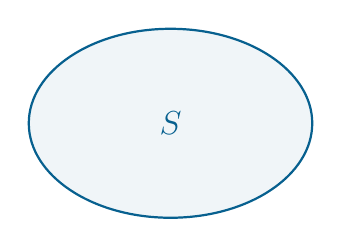
\begin{tikzpicture}
    % (1) Contour for the set S of p-Sylow subgroups
    \fill[figBlue!6] (0, 0) ellipse (1.8 and 1.2);
    \draw[thick, figBlue] (0, 0) ellipse (1.8 and 1.2);

    % (2) Text last
    \node[figBlue, font=\large] at (0, 0) {$S$};
\end{tikzpicture}
\end{center}

\begin{exercise}[Proof of Sylow IV]\label[exercise]{exer:sylow-4-proof}
Prove \cref{thm:sylow-4} by considering the set $S$ of all $p$-Sylow subgroups of $G$ and studying the conjugation action on $S$.
\end{exercise}

\begin{proof}[Proof of \cref{thm:sylow-4} (beyond the lecture)]
Let $S$ be the set of all $p$-Sylow subgroups of $G$, and fix one $p$-Sylow subgroup $P \in S$ (which exists by \cref{thm:sylow-1}). We restrict the conjugation action $G \curvearrowright S$ (given by $g \cdot Q := g Q g^{-1}$) to the subgroup $P \subset G$, obtaining an action $P \curvearrowright S$.

Decomposing $S$ into $P$-orbits with representatives $Q_i \in S$, we have:
\[
|S| = \sum_{Q_i} |\operatorname{Orb}_P(Q_i)|.
\]
By the Orbit--Stabilizer Theorem, each orbit size $|\operatorname{Orb}_P(Q_i)| = \frac{|P|}{|\operatorname{Stab}_P(Q_i)|}$ divides $|P| = p^k$, and is therefore a power of $p$.

We determine which elements $Q \in S$ are $P$-fixed points (i.e., form orbits of size $1$). Clearly, $x P x^{-1} = P$ for all $x \in P$, so $P$ itself is a $P$-fixed point.

Conversely, suppose $Q \in S$ is $P$-fixed, so $x Q x^{-1} = Q$ for all $x \in P$. This means $P \subset N_G(Q)$, where $N_G(Q) := \{ g \in G \mid g Q g^{-1} = Q \}$ is the normalizer of $Q$ in $G$. Note also that $Q \subset N_G(Q)$ (as $q Q q^{-1} = Q$ for all $q \in Q$). Because $|P| = |Q| = p^k$ is the highest power of $p$ dividing $|G|$ and $|N_G(Q)| \mid |G|$, $p^k$ is also the highest power of $p$ dividing $|N_G(Q)|$; hence, $P$ and $Q$ are both $p$-Sylow subgroups of $N_G(Q)$. Applying Sylow III (\cref{thm:sylow-3}) to the group $N_G(Q)$, there exists $g \in N_G(Q)$ such that $P = g Q g^{-1}$. Since $g \in N_G(Q)$, we have $g Q g^{-1} = Q$, and therefore $P = Q$.

Thus, $\{P\}$ is the unique $P$-orbit of size $1$, while every other $P$-orbit in $S$ has size $p^{r_i}$ with $r_i \ge 1$ and is therefore divisible by $p$. Reducing the orbit sum modulo $p$ yields:
\[
|S| = 1 + \sum_{Q_i \neq P} |\operatorname{Orb}_P(Q_i)| \equiv 1 \pmod p.
\]
\end{proof}
\end{content}

\begin{overview}[Summary of Key Concepts]
For a finite group $G$ of order $n = p^k m$ with $p$ prime and $(m, p) = 1$, a subgroup $S \subset G$ of order $|S| = p^k$ is called a \newterm{$p$-Sylow subgroup} of $G$. The lecture established the following results:
\begin{itemize}
    \item \textbf{Sylow I (\cref{thm:sylow-1}):} $G$ contains at least one $p$-Sylow subgroup $S \subset G$ of order $p^k$. This acts as a partial converse to Lagrange's Theorem (whereas the full converse fails, e.g., $A_4$ has order $12$ but no subgroup of order $6$). The proof sets $T = \{ X \subset G \mid |X| = p^k \}$, uses $p \nmid \binom{n}{p^k}$ to find an orbit $\operatorname{Orb}(X_j)$ with $p \nmid |\operatorname{Orb}(X_j)|$, and combines $|\operatorname{Stab}(X_j)| \le p^k$ (via injection $g \mapsto g \cdot a_1$) with the Orbit--Stabilizer Theorem ($p^k \mid |\operatorname{Stab}(X_j)|$) to obtain $|\operatorname{Stab}(X_j)| = p^k$.
    \item \textbf{Sylow II (\cref{thm:sylow-2}):} Every subgroup $H \subset G$ of order $p^\ell$ is contained in some $p$-Sylow subgroup of $G$. Fixing a $p$-Sylow subgroup $P \subset G$ and restricting the left coset action to $H \curvearrowright \frac{G}{P}$ (where $|\frac{G}{P}| = m$ is coprime to $p$) yields an $H$-fixed coset $x P$, giving $H \subset x P x^{-1}$.
    \item \textbf{Sylow III (\cref{thm:sylow-3}):} All $p$-Sylow subgroups of $G$ are conjugate: for any two $p$-Sylow subgroups $P_1, P_2 \subset G$, there exists $x \in G$ with $P_1 = x P_2 x^{-1}$, deduced immediately from the Sylow II argument with $H = P_1$ and $P = P_2$.
    \item \textbf{Sylow IV (\cref{thm:sylow-4}):} The number of $p$-Sylow subgroups of $G$ is congruent to $1 \pmod p$, left as an exercise to prove via the conjugation action on the set $S$ of all $p$-Sylow subgroups.
\end{itemize}
\end{overview}